\section{Game Design}
\label{chap:game_design}

In chapters \ref{chap:design_an_enjoyable_game} - \ref{chap:player_types}, we studied game design principles. This chapter presents how the theories from that study are used in Hover by mapping them to concrete elements in the game. Since Hover is a gamified concept, not all theories are directly relevant. Consequently, only applicable content is mentioned.

\subsection{Reward Systems in Hover}
A suitable reward system is a crucial part of game design, particularly in gamified applications. The theory presented in Chapter \ref{chap:reward_systems} lays the foundation for the rewards implemented in Hover. The goal of the rewards is to facilitate motivation, engagement, and enjoyment. This section presents a description of the forms of rewards used in Hover and the design consideration associated with implementing them. 

\subsubsection{Forms of rewards}
The work of \citeauthor{wang_game_2011}, presented in Chapter \ref{chap:reward_systems}, suggests that games can include eight types of rewards. In Hover, three of these are implemented.

\paragraph*{Score system} 
There are two types of score systems in Hover, namely the points system and the streak system. We consider these to be different types of scores, where both rely on the player’s effort in the game.

The points system lets the players earn points based on the time they have spent tracking. For example, a player training for one hour at a sports center will receive 300 points as a reward. The points are regulated according to the geofence location’s category. Education and social locations generate one point per minute, while cultural and exercise locations generate five points per minute. The distribution of points was structured like this because players are likely to spend more time in social and educational locations than in exercise and cultural ones. 

In the leaderboard, players can see and compare their ranking in the game. The players can filter on both category and time intervals, as seen in Figure \ref{fig:leaderboard_element}.

\begin{figure}[H]
    \centering
    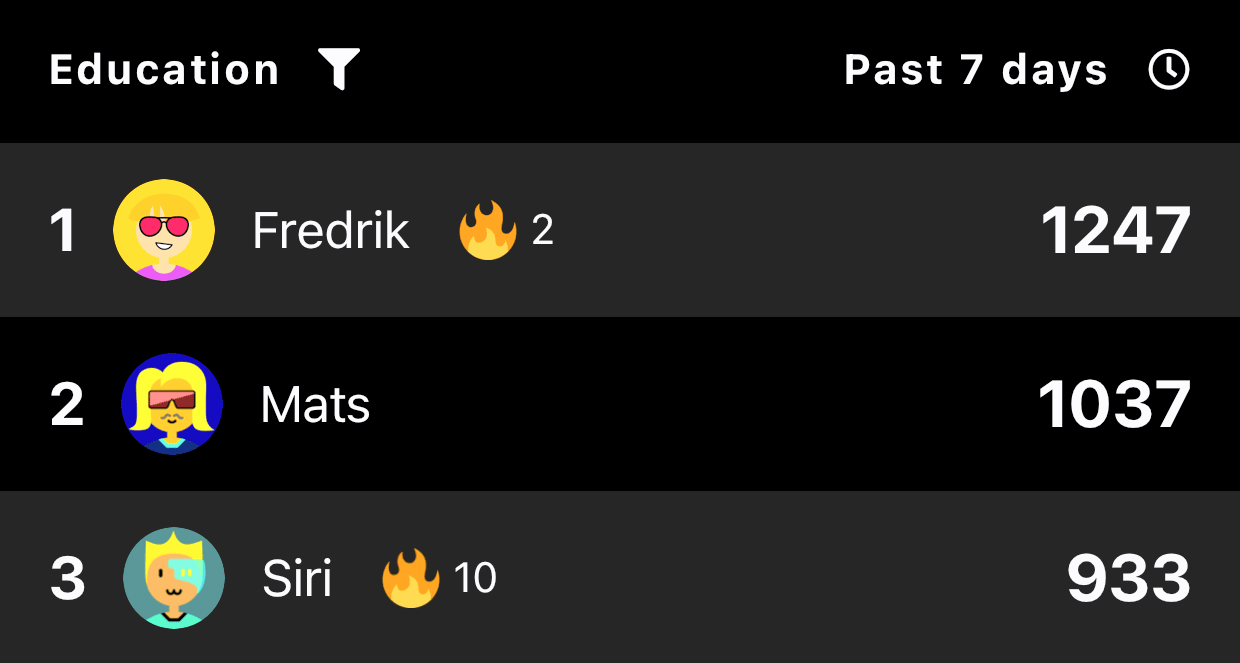
\includegraphics[width=0.65\textwidth]{Images/GameDesign/leaderboard_element.png}
    \caption{Top part of the leaderboard.} 
    \label{fig:leaderboard_element}
    \vspace*{-1\baselineskip}
\end{figure}

The scores are also visible on the players’ profiles. Figure \ref{fig:profile} in Chapter \ref{chap:game_description}, shows how the categories are used as score segments along with the total score. By dividing the categories into different score segments, players can see and compare the scores that matter to them. For instance, players that do not exercise or go to a university will probably not be interested in these scores.

The point system also has a boosting feature that enables cooperation. Players can hover together to get double points during their session. This feature can motivate players to do activities together, engage other players to play, and positively affect the player’s enjoyment. 

The streak system is the second score system in Hover. It counts the number of days in a row that a player has been hovering and is independent of the player’s accumulated points. This particular score system builds on the player’s long-term commitment because the streak is lost if a player goes a day without hovering. The goal of the streak system is to encourage users to do something beneficial every day. The streaks are visible on the leaderboard next to the player’s name, as seen in Figure \ref{fig:leaderboard_element}.

\paragraph*{Achievement systems} 
Another important form of reward is achievement systems. In Hover, achievements are found on the players’ profile as badges (see Figure \ref{fig:profile}). The player’s effort has to meet certain requirements to earn achievements. The types implemented are \textit{score}, \textit{score in category}, and \textit{streak} achievements. In addition to these achievements, players are rewarded with a \textit{first activity} achievement to welcome their first published activity. The achievements are also weighted based on their difficulty. The color of the achievement implies its difficulty level; gold, silver, and bronze (see Figure \ref{fig:achievement_levels}). The difficulty levels are designed to be increasingly hard to get; for instance, \textit{score} achievements are weighted 1000 points for bronze, 5000 for silver, and 15000 for gold. 

\begin{figure}[H]
    \centering
    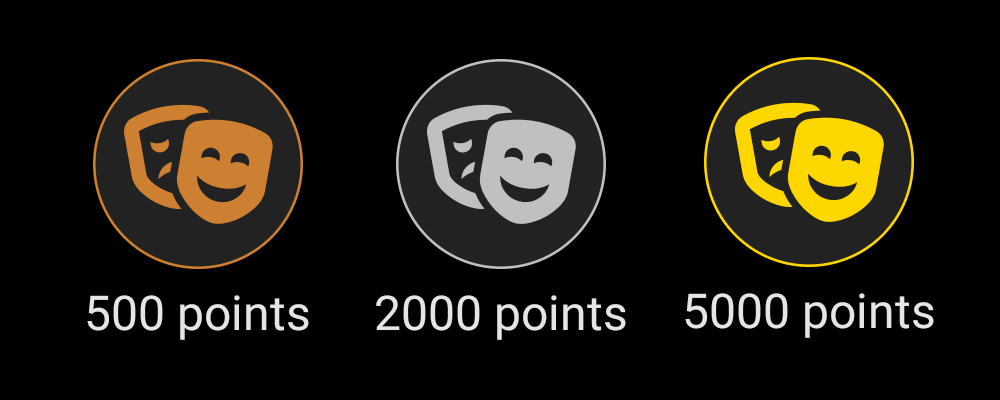
\includegraphics[width=0.6\textwidth]{Images/GameDesign/achievement_levels.png}
    \caption{Achievement’s difficulty level.}
    \label{fig:achievement_levels}
    \vspace*{-1\baselineskip}
\end{figure}

In addition to being visible on the profile, new achievements are published to the feed (as seen in Figure \ref{fig:feed} in Chapter \ref{chap:game_description}). Concrete examples of achievements are "5000 points in the exercise category" and "12-days streak".

\vspace{-0.3\baselineskip}
\paragraph*{Feedback messages} 
The last type of reward implemented in Hover is feedback messages. Players are given feedback before, during, and after hovering, both when the app is foregrounded and backgrounded. Animations, emojis, colors, and sounds are used to give feedback.

When players complete an activity or invite others to a challenge, they are prompted with feedback messages that appear as a confirmation message (see figures \ref{fig:feedback_activity} and \ref{fig:feedback_challenge}). The messages are decorated with emojis to make them more playful and positive.
 
\begin{figure}[H]
    \centering
    \begin{subfigure}[b]{0.46\textwidth}
        \centering
        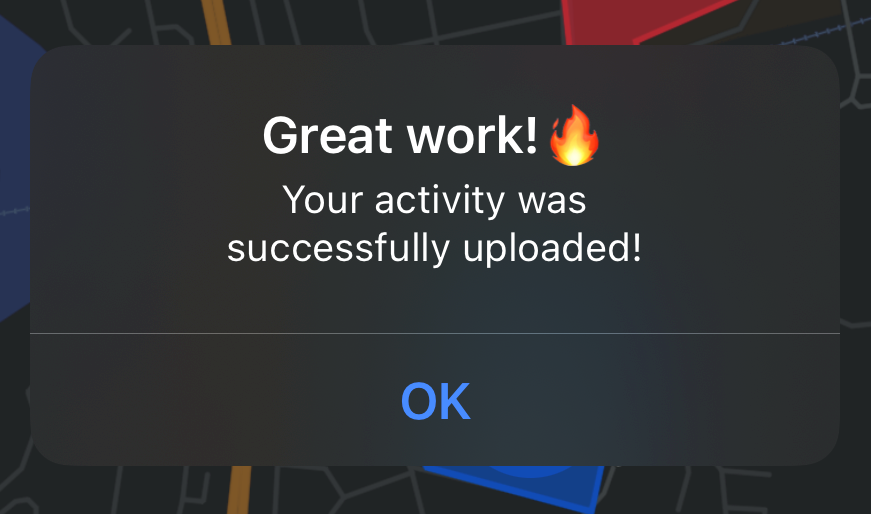
\includegraphics[width=\textwidth]{Images/GameDesign/feedback_activity.png}
        \caption{Activity feedback.}
        \label{fig:feedback_activity}
    \end{subfigure}
    \quad
    \begin{subfigure}[b]{0.36\textwidth}
        \centering
        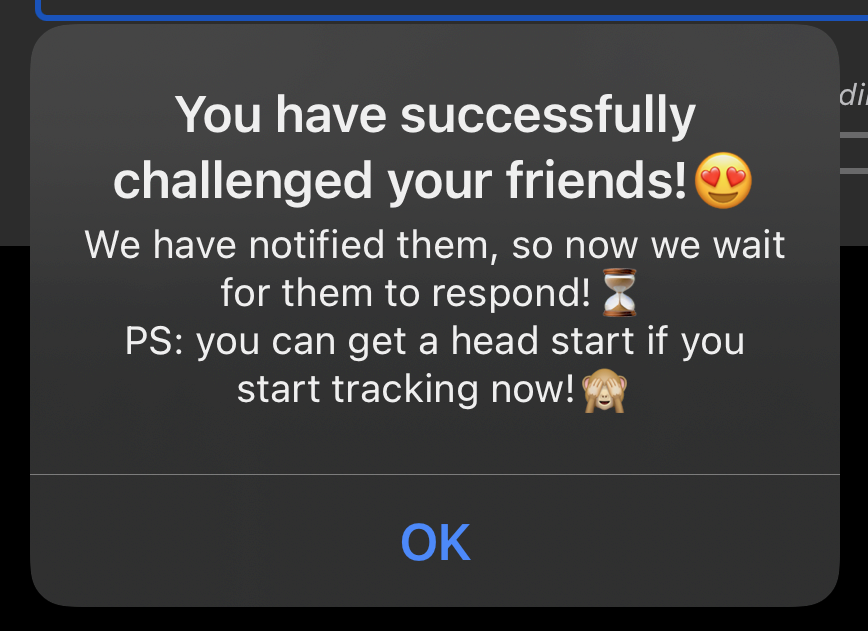
\includegraphics[width=\textwidth]{Images/GameDesign/feedback_challenge.png}
        \caption{Challenge feedback.} 
        \label{fig:feedback_challenge}
    \end{subfigure}
    \caption{Feedback messages.}
    \vspace{-\baselineskip}
\end{figure}
 
\subsubsection{Reward Design considerations}
\citeauthor{wang_game_2011}’s article on reward systems presents seven design considerations for developing reward systems. Four of these was directly relevant to us during the development of Hover:

\paragraph*{Balance} 
Time spent on activities and the points given needs to be balanced. The players will experience the game as frustrating if not enough points are rewarded and boring if too many points are rewarded, for the activities they complete. As mentioned above, it is easier to spend eight hours on campus than be at a sports center training for eight hours. Thus the points should be distributed based on the geofence category (culture, education, exercise, and social). A consequence of this is that the points will not change based on the experience but rather on effort. Hence, experienced players might feel that it is easier to earn points than beginners because there is no increase in difficulty.

The balance between player experience and difficulty is incorporated in the achievement system. The three achievement levels, \textit{bronze}, \textit{silver}, and \textit{gold}, are designed to be increasingly more difficult to earn. This balance gives the player an incentive to strive for the next achievement level because it is not too easy nor too hard to achieve. 

The three rewards systems in Hover facilitate three ways of advancing, as compared in Table \ref{tab:rewardsystems_balance}. The \textit{point system} lets the player climb the leaderboard; however, points are partly volatile and non-volatile. The \textit{streak system} is volatile and requires a committed and consistent player, while the \textit{achievement system} is non-volatile. The balance between volatile and non-volatile rewards ensures that the player always has something to fall back on when returning to the game.

\begin{table}[H]
    \centering
    {\renewcommand{\arraystretch}{2}%
    \begin{tabular}{| p{0.16\textwidth} | p{0.37\textwidth} | p{0.38\textwidth} |}
        \hline
        \multicolumn{1}{|l|}{}   & \multicolumn{1}{c|}{\textbf{Volatile reward}} & \multicolumn{1}{c|}{\textbf{Non-volatile reward}} \\ \hline
        \textbf{Point system}    & Leaderboard focuses on the \textit{Last 7 days}, and points are out of focus after a week. & The player’s all-time points are shown on their profile. Players can filter on pre-defined time intervals to find other score segments on the leaderboard. \\ \hline
        \textbf{Streak system}   & Streaks are lost if a player goes a day without hovering.     &   \\ \hline
        \textbf{\small Achievement system} &     & Once acquired, the player has permanently earned the achievement.   \\ \hline
    \end{tabular}}
    \caption[Categorizing the three types of rewards in Hover]{Categorizing the three types of rewards in Hover as volatile and non-volatile.}
    \label{tab:rewardsystems_balance}
    \vspace*{-0.5\baselineskip}
\end{table}

There are benefits derived from utilizing multiple reward systems. One is that competitiveness can be captured amongst players in different spectrums of the experience scale. Another one is the ability to create a competitive environment between players of similar experience levels.

\paragraph*{Uncertainty and secrecy} 
Uncertainty and secrecy are necessary to impose curiosity in a game. In Hover, the achievements are somewhat hidden. Through the player profile, players can view their earned achievements and progress toward the next (see Figure \ref{fig:unachieved_levels}). However, detailed information such as the name and the requirements for the achievements are hidden. Instead, a progress bar gives intrinsic feedback on their progress towards the new achievement. By utilizing secrecy, players have to put in work and use their imagination to reveal the achievement. 

\begin{figure}[H]
    \centering
    
\includegraphics[width=0.7\textwidth]{Images/GameDesign/unachieved_levels.png}
    \caption{Progress towards new achievements.}   
    \label{fig:unachieved_levels}
    \vspace*{-\baselineskip}
\end{figure} 

\paragraph*{Social purpose} 
The social aspect is crucial in Hover because it gives purpose to the points and the achievement. Players' social status is based on the accumulated rewards that are shared with other players. Points, streaks, progress, and achievements are visible in the feed, the leaderboard, and the player profiles. This focus on social status enhances competitiveness and gives players incentive. The playing frequency revealed by the streak and the hard-to-get achievements distinguishes advanced and casual players. These types of rewards also serve as a symbol to increase unity between skilled players.

\subsection{Player Types in Hover}
The seven dimensions of player types found in \citet{hamari_player_2014} primarily focus on online games. However, the categories are still valid for gamification concepts like Hover. Hover’s players will presumably have different interests and motivations for engaging in the game. Therefore, they will not be categorized as one player type but rather as a combination of the seven dimensions.

According to \citet{hamari_player_2014}, the dimension of \textit{achievement} focuses on single-oriented players. Achievers will likely be present in Hover because of the reward systems. The mechanisms used in these systems can motivate, track progress, allow accumulation of badges, and contribute to in-game status. \citet{yee_motivations_2007} suggested that achievers are likely to respond to game elements that measure the players’ performance, for instance, progress bars, streaks, leaderboards. In Hover, these measurable mechanics are implemented in the \textit{unachieved achievements} screen, the \textit{ongoing challenges} screen and the \textit{leaderboard} (see figures \ref{fig:challenge}, \ref{fig:leaderboard}, and \ref{fig:achievements} in Chapter \ref{chap:game_description}).
    
The \textit{sociability} dimension focuses on community-oriented players. Hover is a community-based game that facilitates social interaction through reactions, hovering with friends, and competing in challenges. Reactions are a social reward mechanism that gives socializers a reason to engage because they can motivate players, express support, and increase in-game status. Socializers often have an interest in viewing other players, and Hover enables this through the feed, the ongoing challenges, the leaderboard, and the player profiles. Viewing other players’ activities can also have a motivating effect and inspire them to do new interesting activities. 

Though the dimension of \textit{exploring} is not too prominent in Hover, viewing other player’s activities, exploring unachieved achievements, and finding new locations on the map can be regarded as exploring.

The leaderboard in Hover enables the dimension of \textit{domination} because some players enjoy dominating the leaderboard. Many MMORPGs have various aspects of domination, such as provocative behavior. However, domination for players in Hover is more concerned with getting more points than their friends. Some players might only take an interest in dominating specific categories, such as education and health. For that reason, enabling leaderboard-filtering on categories and time intervals enhances the experience of domination.

\subsection{Use of Malone’s Theories on Intrinsic Motivation}
Malone’s "What Makes Things Fun to Learn?" article presents three essential elements in his article: challenge, fantasy, and curiosity. All of them are, to some degree, related to Hover’s game design.

\paragraph*{Challenge}
For a game to be enjoyable, appropriately designed challenges are necessary. As mentioned in the section describing reward systems earlier in this chapter, the game must balance difficulty and player experience in the score and achievement systems.

Another aspect of the game, which is not mentioned in the reward systems section, is the importance of an appropriate degree of challenge in the "in-game challenges" where users compete against each other. Since the creator can customize the in-game challenges, they can select an appropriate difficulty based on previous experience. Additionally, ongoing in-game challenges have hidden information and a goal. 

\begin{wrapfigure}{r}{0.53\textwidth}
    \vspace{-0.8\baselineskip}
    \hspace*{0.03\textwidth}
    \begin{minipage}{0.49\textwidth}
        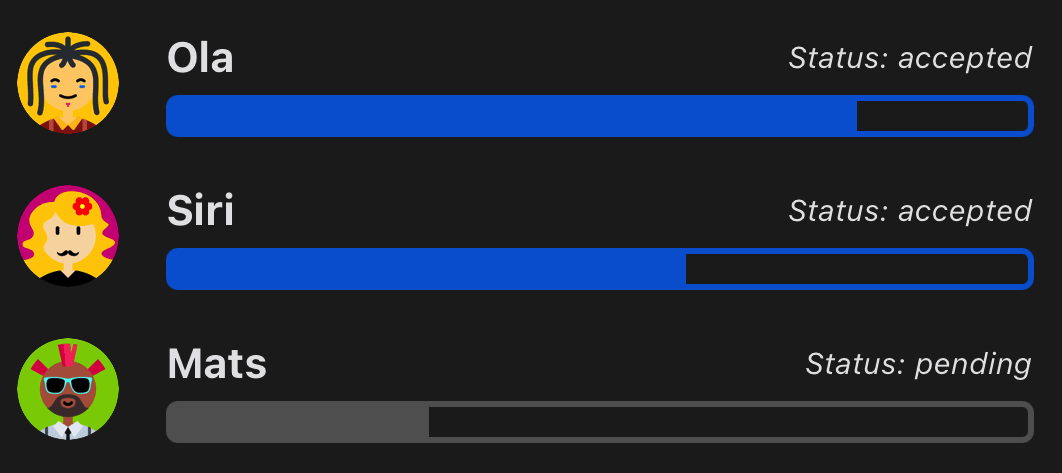
\includegraphics[width=\textwidth]{Images/GameDesign/challenge_progress.png}
        \caption{Challenge progress.}
        \label{fig:challenge_progress}
        \vspace*{-0.8\baselineskip}
    \end{minipage}
\end{wrapfigure}

Players do not precisely know their progress. Instead, the description and the progress bar give the player a clear goal and indicate their progress (see Figure \ref{fig:challenge} in Chapter \ref{chap:game_description}). The progress is also not updated before the player publishes a new activity. Therefore, players cannot be entirely sure if they are leading the in-game challenge or not. Hiding details and information like that gives uncertain outcomes, which balances the difficulty. 

\paragraph*{Fantasy}  
Fantasy in games makes them more appealing. In Hover, players have an avatar representing them. The avatars are randomly generated; however, players can regenerate until they find an avatar they like. Examples of avatars are illustrated in Figure \ref{fig:avatar_collage}. The avatar creates an extrinsic fantasy where players accumulate points for their avatar.

\begin{figure}[H]
    \centering
    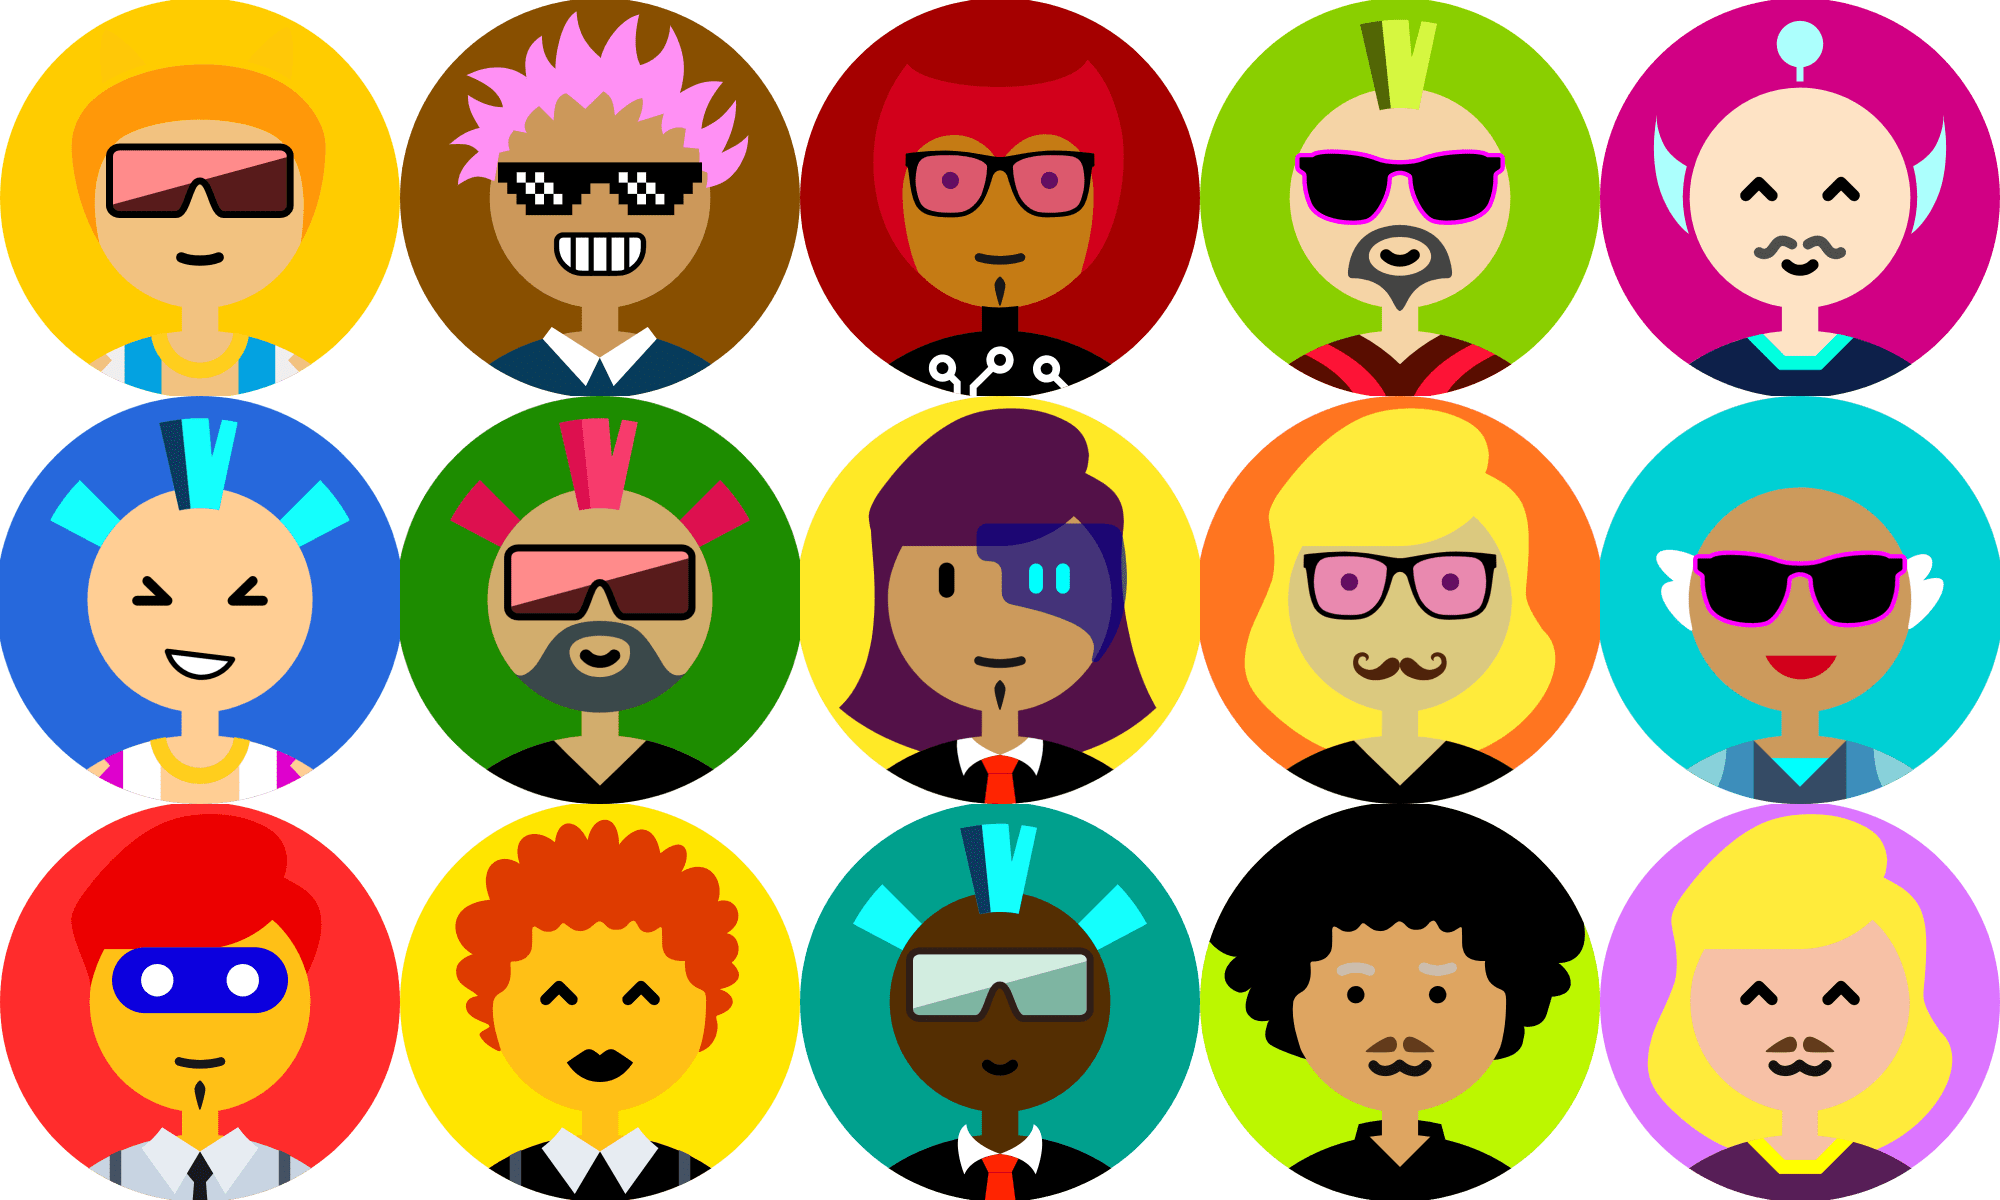
\includegraphics[width=0.85\textwidth]{Images/GameDesign/avatar_collage.png}
    \caption{Player avatar examples.}
    \label{fig:avatar_collage}
    \vspace{-0.5\baselineskip}
\end{figure}


\paragraph*{Curiosity} 
Curiosity is a central element in game design used to encourage exploration and draw players’ attention. Curiosity was mentioned in the game reward systems section under the "uncertainty and secrecy as a design consideration" part. According to \citeauthor{malone_what_1980}, this type of curiosity can be categorized as cognitive curiosity, which is one of two elements of curiosity. In Hover, cognitive curiosity is found in the achievement system. Since the requirements of the unachieved achievements are hidden from the player, they may be triggered by their curiosity to explore that achievement further. 

Sensory curiosity is mentioned as the other category of curiosity. Particular graphical elements, sounds, and similar attract the player’s attention. In Hover, sensory curiosity is present as decoration and as a representation system. Icons, emojis, and colors are used throughout the application to decorate the game elements and feedback messages. 

For the representation system, progress bars are used to represent the progress toward the next point while tracking. Hence the progress bar represents the time it takes between points, instead of using text. If the player moves outside the geofence, the progress bar stops moving to illustrate that the tracking has paused (see Figure \ref{fig:tracking_progressbar_paused}).

\begin{figure}[H]
    \centering
    \begin{subfigure}[b]{0.48\linewidth}
        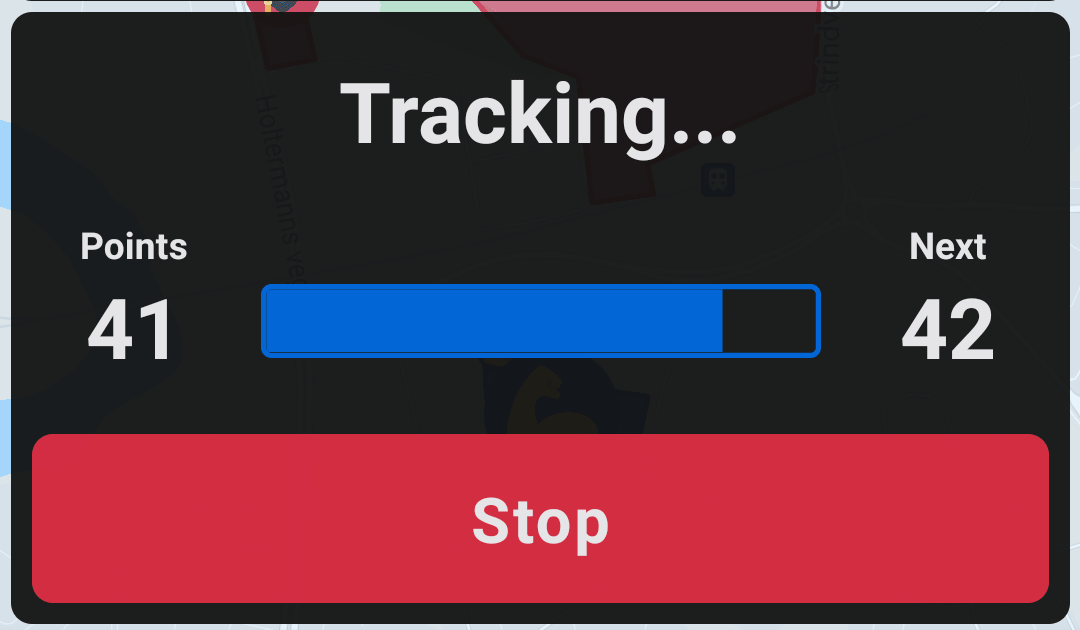
\includegraphics[width=\textwidth]{Images/GameDesign/tracking_progressbar.png}
        \caption{Tracking in progress.}
        \label{fig:tracking_progressbar}
    \end{subfigure}
    \quad
    \begin{subfigure}[b]{0.48\linewidth}
        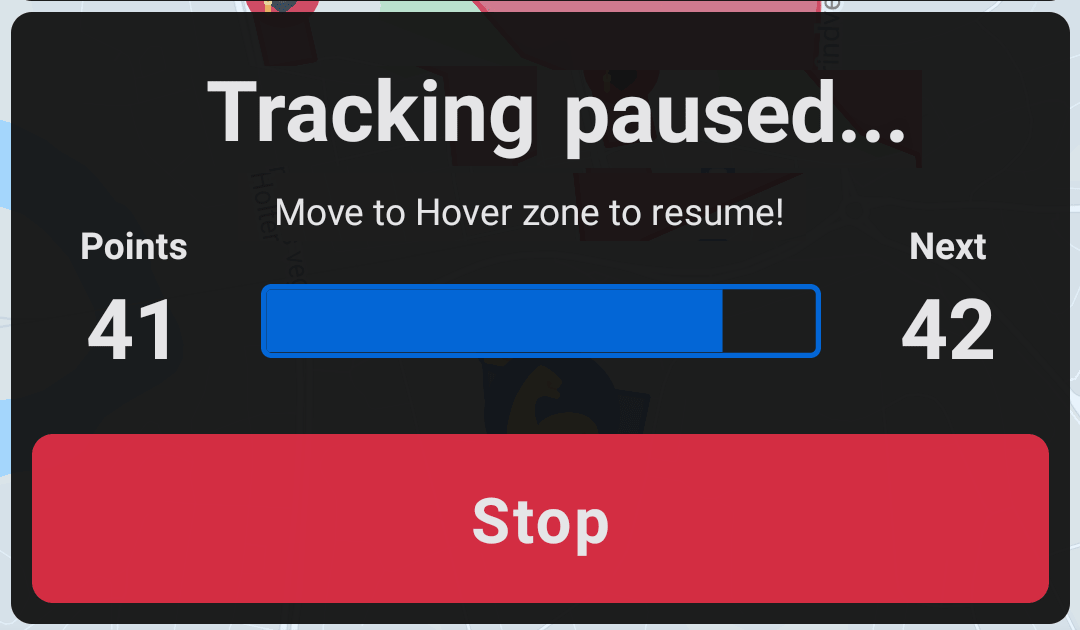
\includegraphics[width=\textwidth]{Images/GameDesign/tracking_progressbar_paused.png}
        \caption{Tracking paused.}
        \label{fig:tracking_progressbar_paused}
    \end{subfigure}
    \caption{The progress bar, used as a representation system for time.}
    \vspace{-0.5\baselineskip}
\end{figure}

Furthermore, to start tracking, players have to be located within a geofence. To indicate that tracking is restricted to valid hover zones, gray and green buttons are used to illustrate whether this functionality is disabled or not. 

\begin{figure}[H]
    \centering
    \begin{subfigure}[b]{0.48\linewidth}
        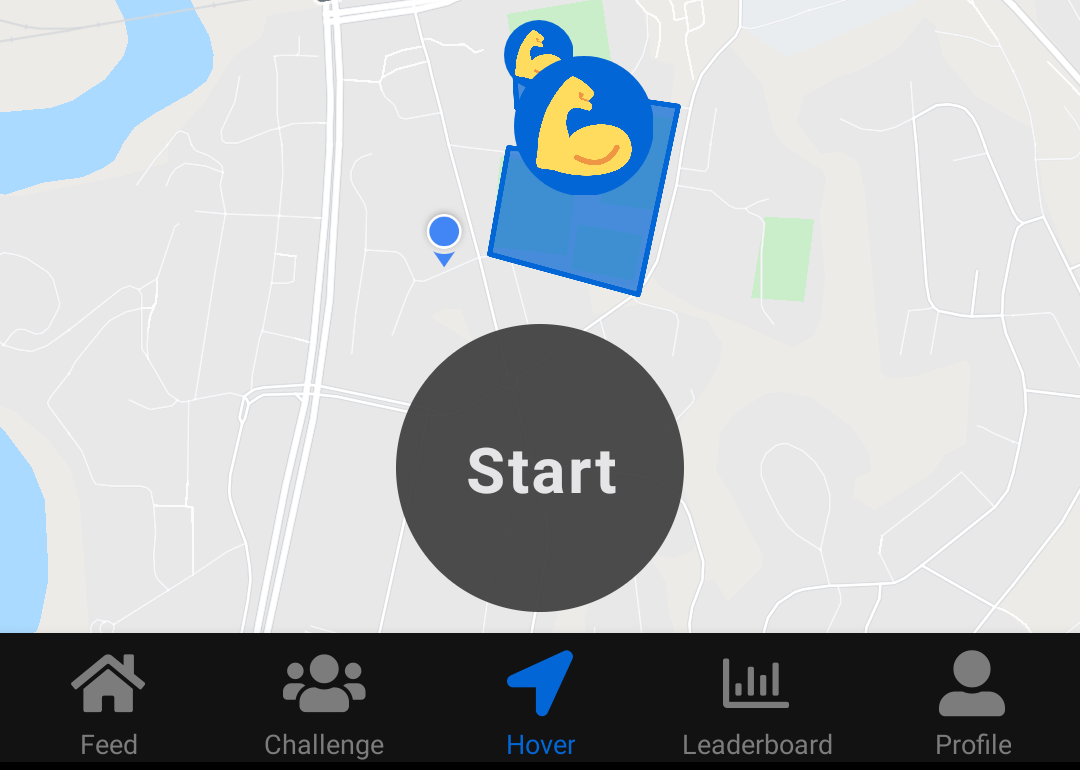
\includegraphics[width=\textwidth]{Images/GameDesign/map_button_disable.png}
        \caption{Hovering disabled.}
        \label{fig:map_button_disable}
    \end{subfigure}
    \quad
    \begin{subfigure}[b]{0.48\linewidth}
        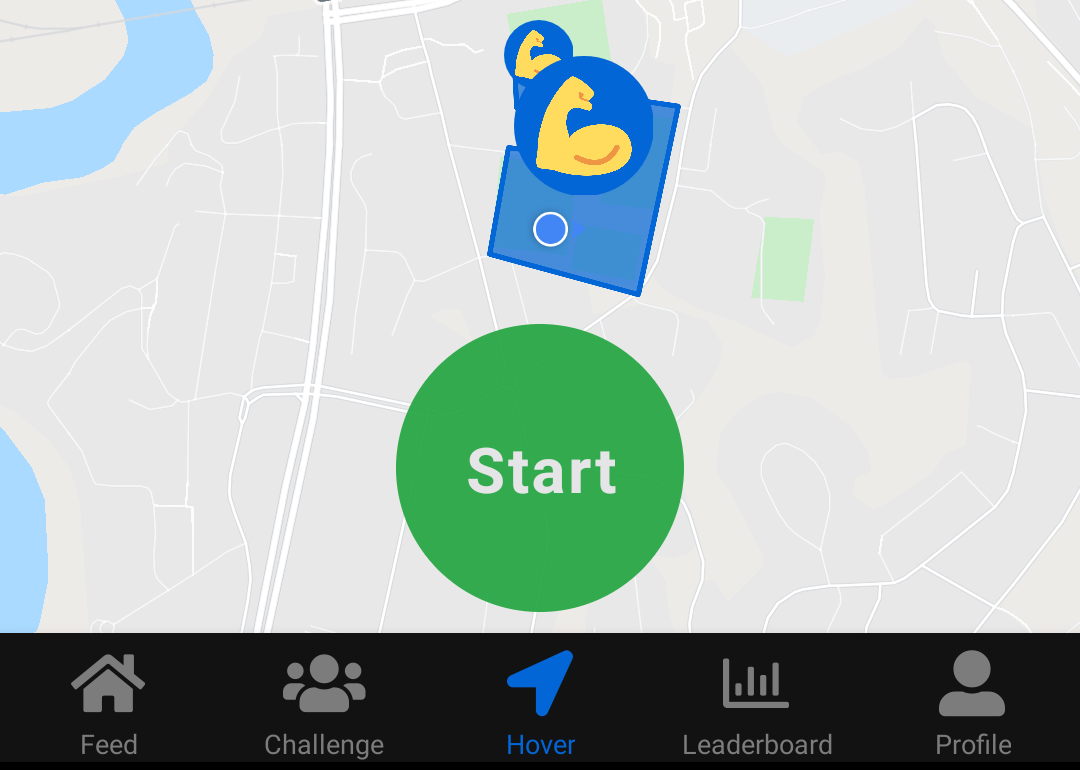
\includegraphics[width=\textwidth]{Images/GameDesign/map_button_enable.png}
        \caption{Hovering enabled.}
        \label{fig:map_button_enable}
    \end{subfigure}
    \caption{The \textit{Start} button when the user is outside and inside a Hover zone.}
    \vspace{-0.5\baselineskip}
\end{figure}

\subsection{Use of the GameFlow Framework}
The concept of flow, described in the GameFlow article by \citeauthor{sweetser_gameflow_2005}, is to some degree applicable to Hover. Since Hover is a gamification concept and not a conventional game, some elements are not relevant. Many of the GameFlow elements correlate with aspects mentioned earlier in this chapter, and consequently, these will only be discussed briefly here.

\paragraph*{Challenge and Player Skills} 
Both of these aspects have been mentioned earlier, but to summarize, a central consideration in game design is to balance challenge and player skill. The challenge in a game must not be too hard or too easy. Such games will create frustration and boredom, respectively, decreasing player engagement. In Hover, this balance is vital in the achievement system because players should be rewarded according to their effort.

Another aspect related to the concept of challenge is the in-game challenges that players can invite to and participate in. Since the players themselves define the rules, it can be difficult for them to understand what the challenge requires them to do. Thus, a description is generated to give the player a better understanding of what a challenge requires during the creation process (see Figure \ref{fig:challenge_description_close}).

\begin{figure}[H]
    \centering
    
\includegraphics[width=0.6\textwidth]{Images/GameDesign/challenge_description_close.png}
    \caption{Challenge description, generated from the rules defined by the player.}
    \label{fig:challenge_description_close}
    \vspace{-0.5\baselineskip}
\end{figure}

\paragraph*{Control} 
Control is also a central element of game design; players should feel a sense of control over their actions in the game and transfer their intentions to in-game behavior. 
To incorporate the element of control in Hover, it was essential to design and build intuitive user interfaces. We followed common design principles and patterns. Examples include utilizing a horizontal process flow when creating challenges and tracking (see figures \ref{fig:create_challenge_flow} and \ref{fig:tracking_flow} in Chapter \ref{chap:game_description}). Utilizing such a flow can provide a sense of progress. Additionally, players cannot proceed to the next step in the flow before all sub-steps are finished, indicated by using disabled "Next"-buttons.

Furthermore, \citet{sweetser_gameflow_2005} also suggests that players should be able to recover from their mistakes; thus, the game should support this. If a player mistakenly kills the app while hovering, Hover automatically resumes tracking on restart. This particular functionality lets players recover from a mistake that would otherwise cause players to lose their activity and disturb the gameplay. Another mechanism that lets players recover from mistakes is that players may resume or discard their activities when tracking is stopped, as illustrated in Figure \ref{fig:activity_control}. 

\begin{figure}[H]
    \centering
    
\includegraphics[width=0.68\textwidth]{Images/GameDesign/activity_control.png}
    \caption{Resume or discard activity selection.}    
    \label{fig:activity_control}
    \vspace{-0.5\baselineskip}
\end{figure}


\paragraph*{Clear goals} 

\begin{wrapfigure}{r}{0.44\textwidth}
    \centering
    \vspace*{-1.6\baselineskip}
    \hspace*{0.03\textwidth}
    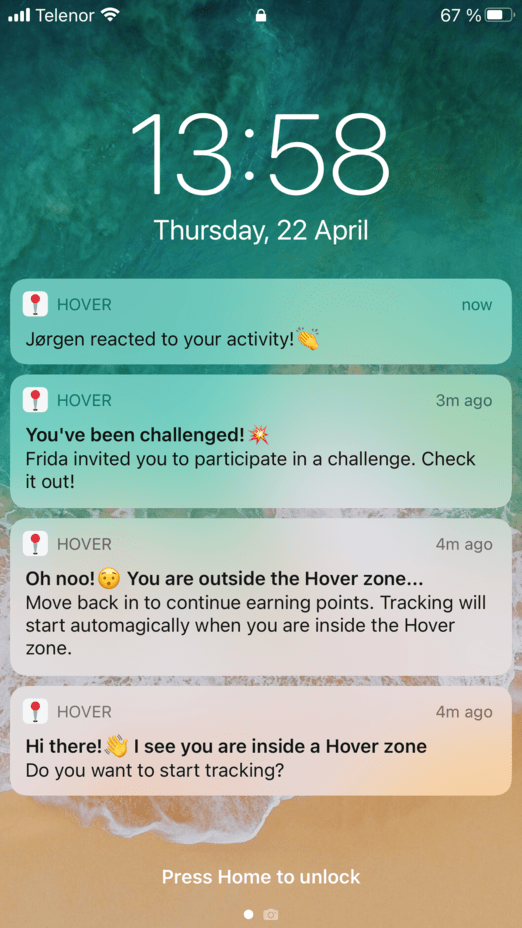
\includegraphics[width=0.4\textwidth]{Images/GameDesign/push_notifications.png}
    \caption{Examples of push notifications used in Hover.}
    \label{fig:push_notification}
     \vspace*{-1.4\baselineskip}
\end{wrapfigure}

Clear goals in games are essential to improve player engagement. In Hover, the main goal is to accumulate points while hovering. Consequently, the application launches to the "Hover screen" (Figure \ref{fig:tracking_flow} in Chapter \ref{chap:game_description}) to encourage players to start hovering if they are inside a valid zone. Additionally, players receive a push notification when they enter a valid hover-zone, as shown in the bottommost notification in Figure \ref{fig:push_notification}.

Moreover, the concept of clear goals is also used for the challenges. All challenges include a generated description of the challenge’s rules (as illustrated in Figure \ref{fig:challenge_description_close}).

\clearpage
\paragraph*{Feedback} 
As briefly described in the reward system section, feedback is vital as a reward. Moreover, \citeauthor{sweetser_gameflow_2005} also suggests that feedback is important to improve player enjoyment. In Hover, players can always see their score and progress, both while they are tracking and not tracking.

Feedback is essential while hovering to ensure that the players understand whether or not they receive points (inside or outside the zone) at all times. Thus, players get either visual or textual feedback when they have left a zone or when they have started a "Hover with friend" session (see figures \ref{fig:tracking_progressbar_paused} and \ref{fig:friend_tracking}).

\begin{figure}[H]
    \centering
    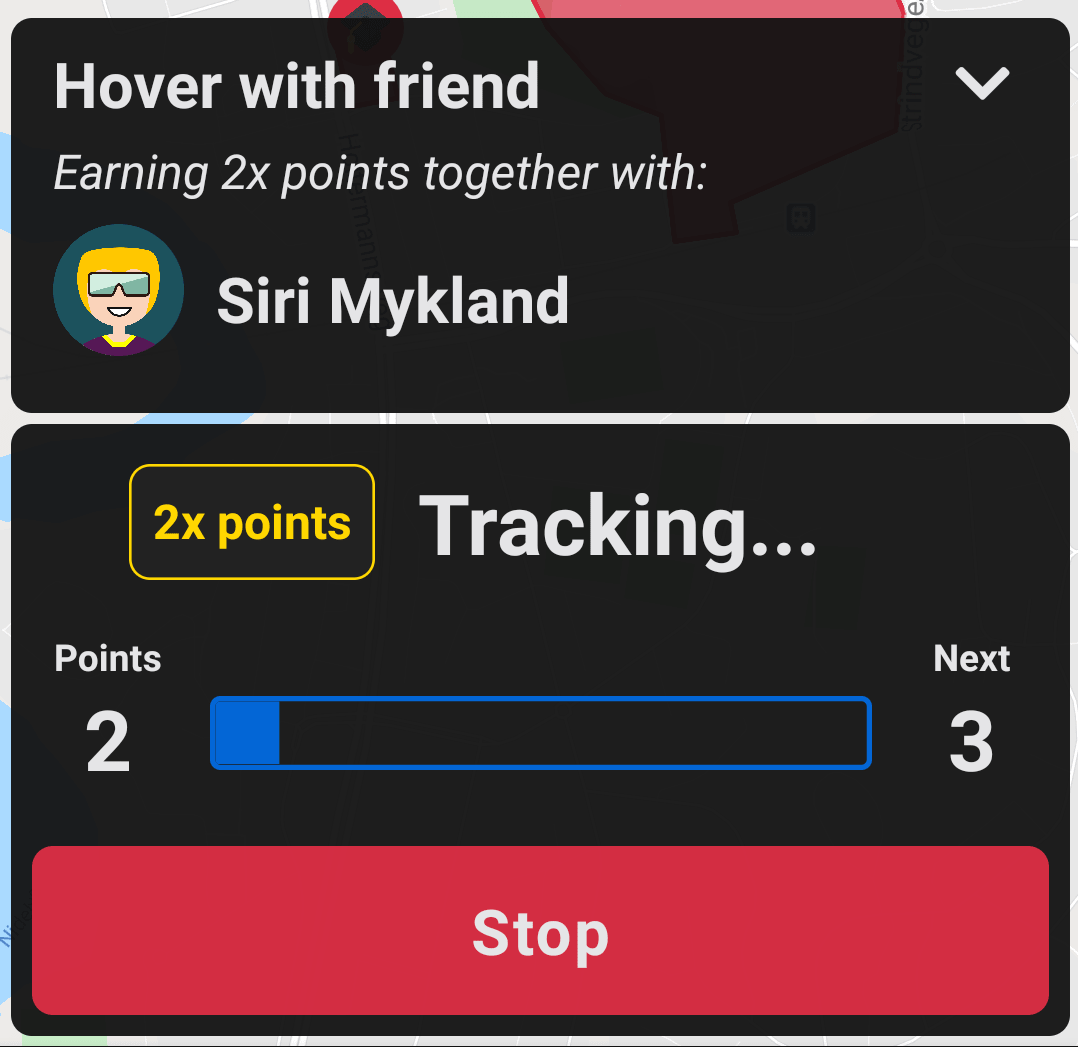
\includegraphics[width=0.60\textwidth]{Images/GameDesign/friend_tracking.png}
    \caption[Hover with friend]{Hover with friend, indicated by "2x points", player name, and avatar.}
    \label{fig:friend_tracking}
\end{figure}

In addition to in-game feedback, players are given push notifications on their location status (inside or outside a geofence), updates on challenges (invites, responses, wins, and loses), and rewards (achievements and reactions). These push notifications are decorated with emojis to be more playful and informative. The third notification in Figure \ref{fig:push_notification} gives direct feedback that suggests that the player should move back into the area. The message is also an indirect reminder for them to publish their activity when they leave a location.

\paragraph*{Social Interaction} 
Interaction between players was discussed in the social purpose part of the reward systems section and in the player types section. Social interaction in games increases player engagement and fun in a game, enhancing the purpose of the game. Hover includes competitive and cooperative interaction through the challenges and friend-tracking features. In addition to this, players can interact by showing support through reacting to each others’ activities and achievements. The game’s meaning is also improved by including the possibilities to share achievement and compare points against friends.

\subsection{Summary}
This chapter has described Hover’s game design based on the theories from chapters \ref{chap:design_an_enjoyable_game}, \ref{chap:reward_systems}, and \ref{chap:player_types}. Reward systems, player types, the use of Malone’s theories, and elements from the GameFlow framework have been presented. The next chapter describes Hover’s functional requirements.